\part{The Graph Abstract Data Type}
\label{ch:graphadt} 

\chapter{Graph definitions} %-------------------------------------------------
\label{sec:graphdefs}
Graphs are important and general mathematical objects that are widely used in theory and practice. 
They distill the basic idea of a relationship among a set of objects. 
Informally we can think of a graph as a collection of dots (the set of objects) with lines connecting them (describing the relationship). 
The lines can be either directed (arrows) or undirected.

We are interested in the algorithmic aspects of graph theory (``how can we do it efficiently and systematically?").  
To talk about this precisely, we must start with precise definitions.

\begin{Definition}\label{def:digraph} 
A \defnfont{digraph} $G=(V,E)$ is a  finite nonempty set $V$ of \defnfont{nodes} 
together with a (possibly empty) set $E$ of ordered pairs of nodes of $G$ called \defnfont{arcs}. 
Digraph stands for \boldfont{di}rected \boldfont{graph}.
\end{Definition}

\begin{Boxample}[0] \label{ex:digraph}
For the digraph shown, write down the sets $V$ and $E$.\\
\newline 
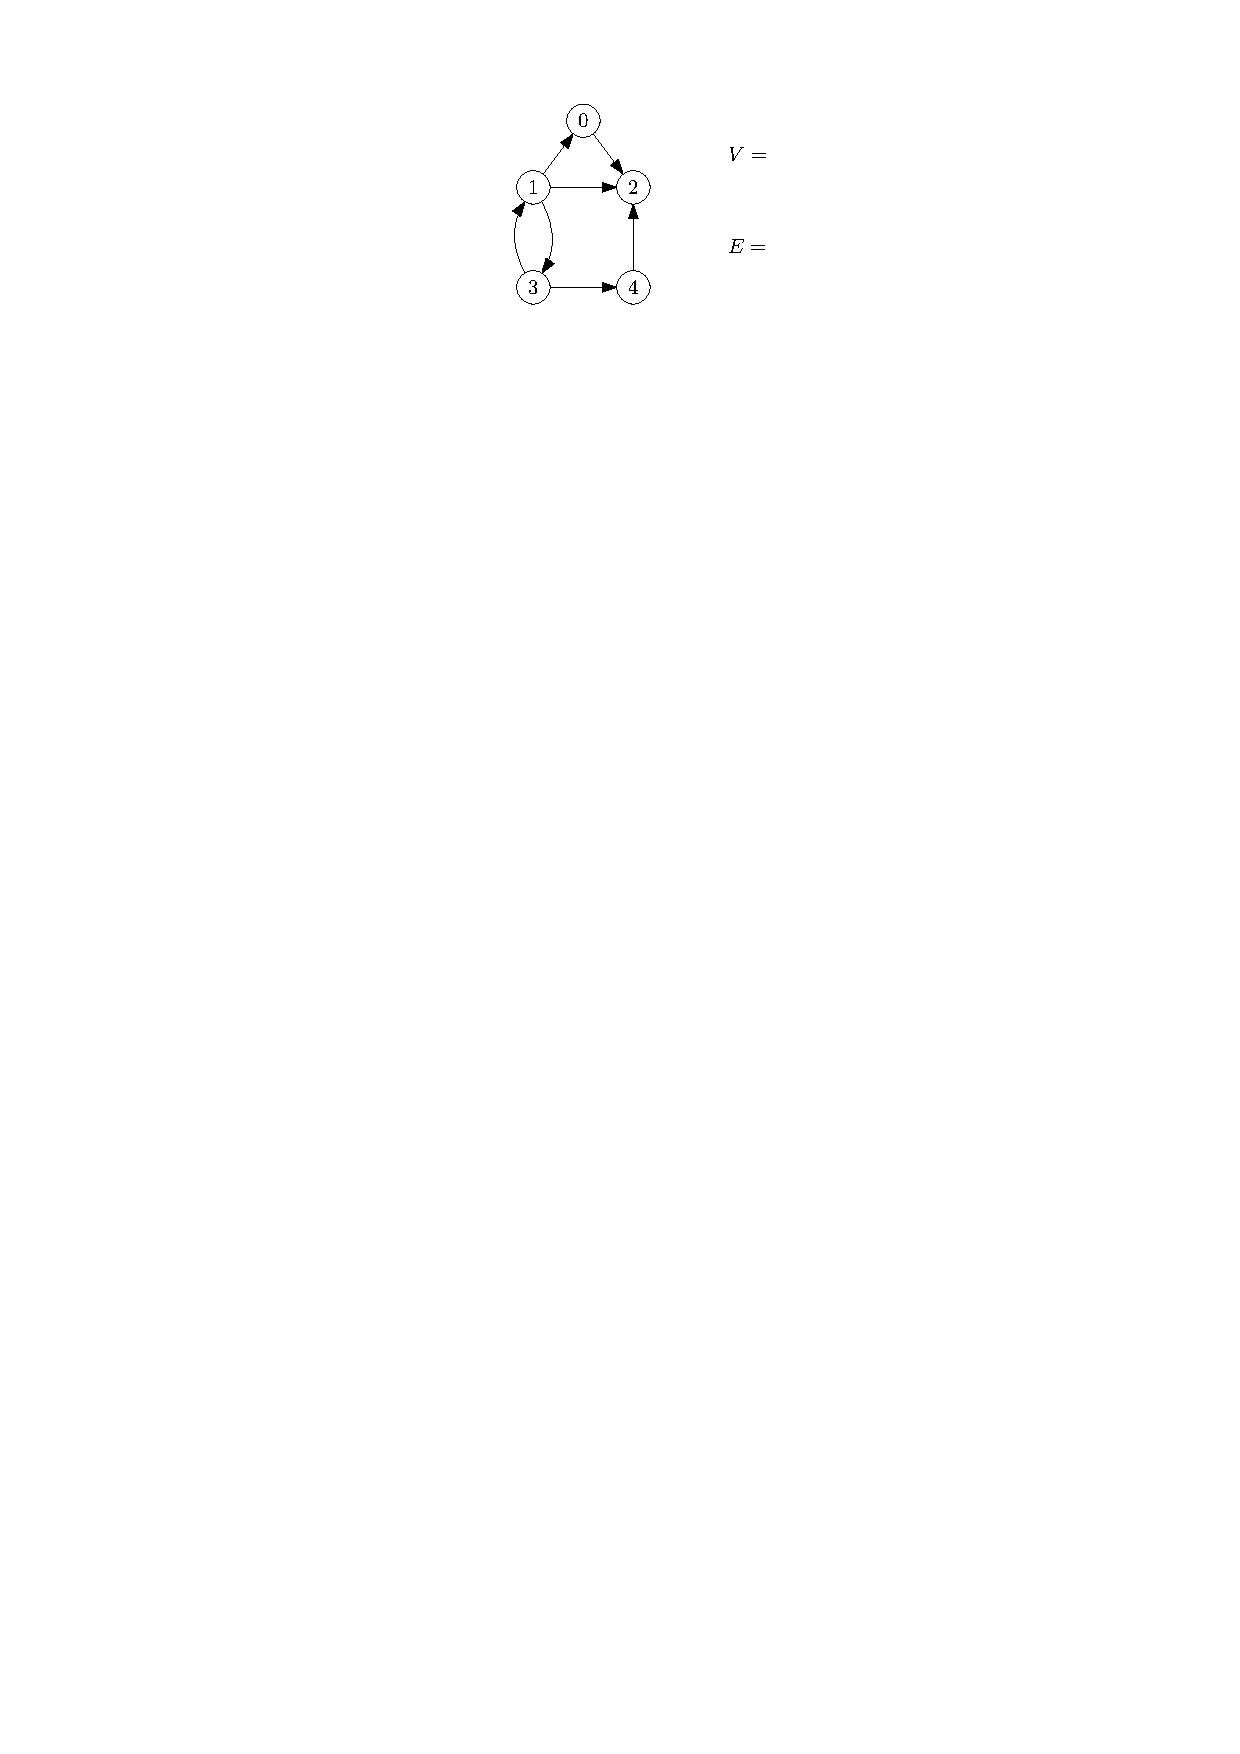
\includegraphics{graphExDirectedVE}
\end{Boxample}

\begin{Definition}\label{def:graph}
A \defnfont{graph} $G = (V, E)$ is a finite nonempty  set $V$ of 
\defnfont{vertices} together with a (possibly empty) set $E$ of unordered
pairs of vertices of $G$ called \defnfont{edges}. 
Note that the singular of vertices is \defnfont{vertex}.
\end{Definition}

\begin{Boxample}[1] \label{ex:graph}
For the graph shown, write down the sets $V$ and $E$.\\
\newline 
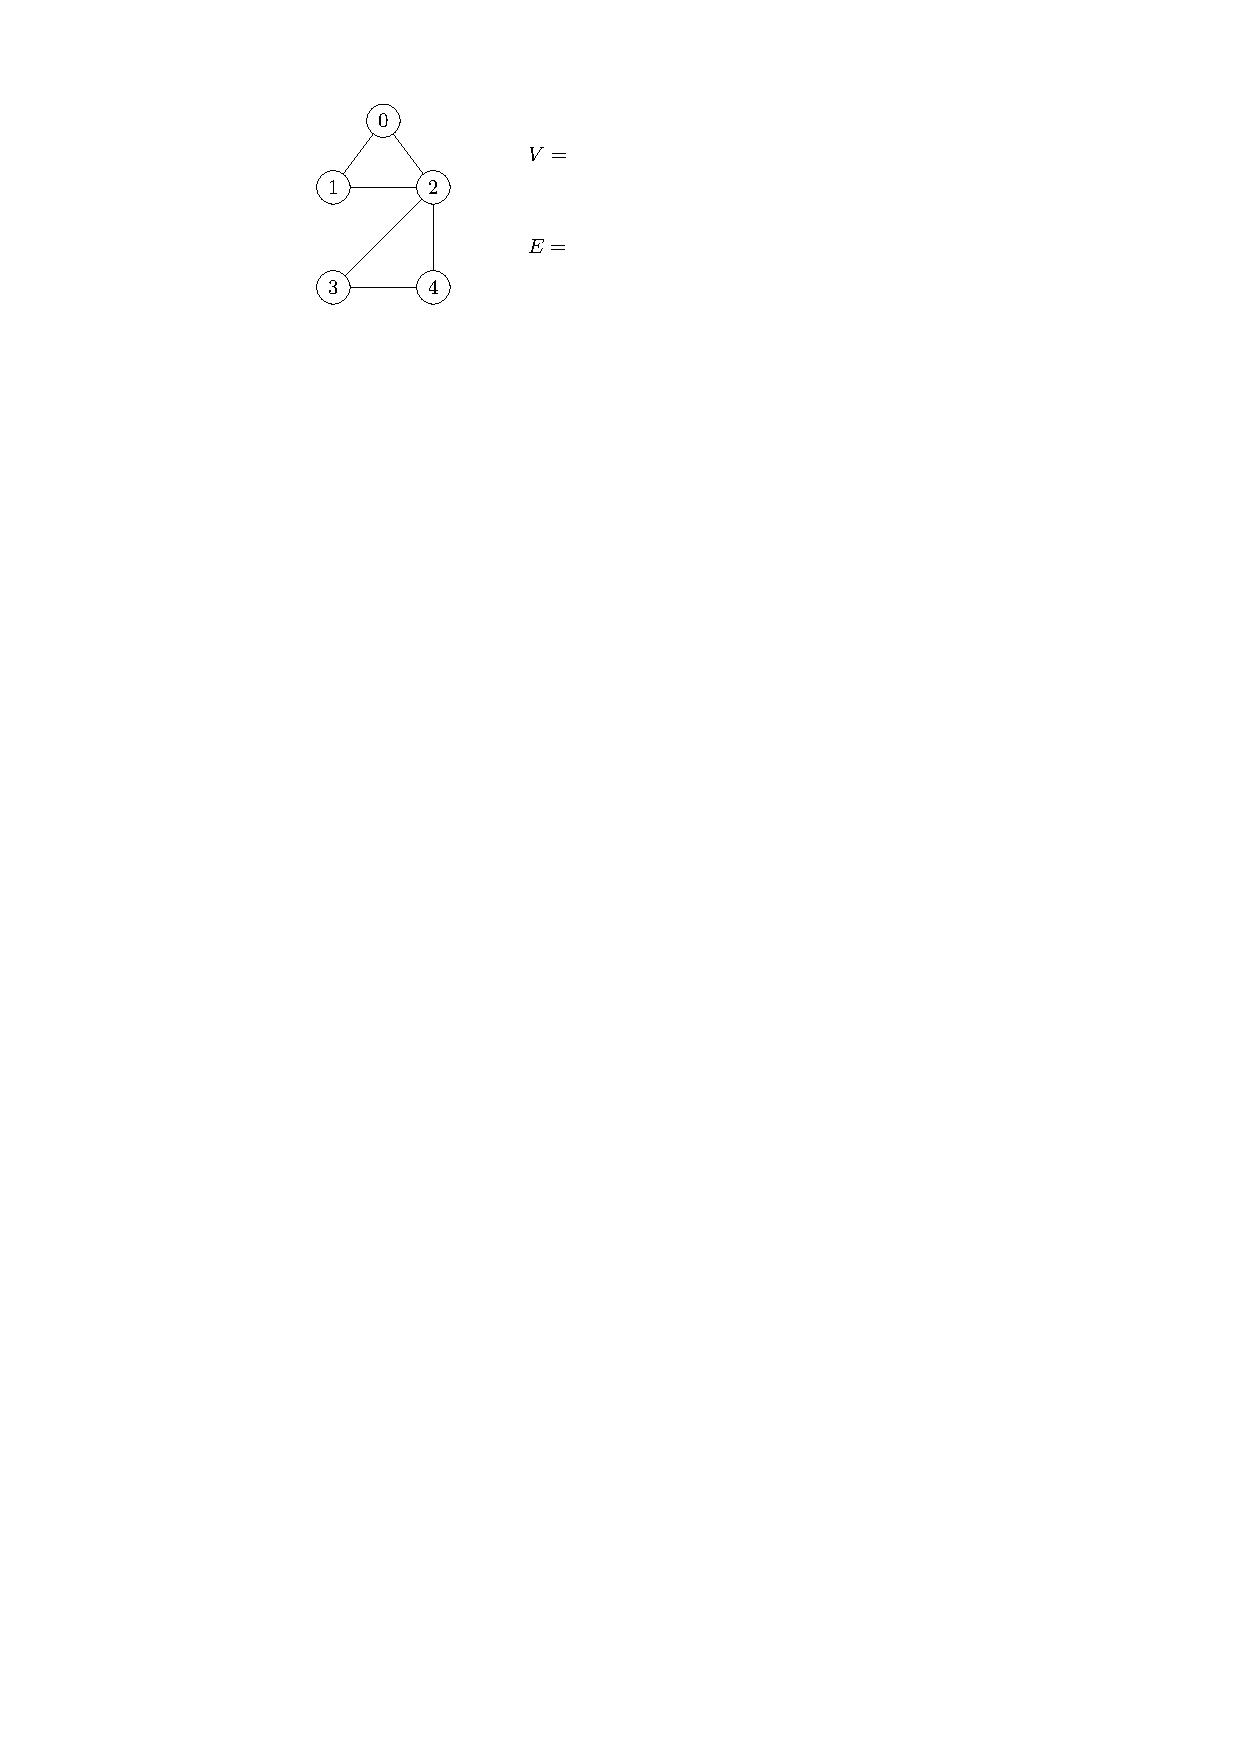
\includegraphics{graphExUndirectedVE}
\end{Boxample}

Some notes on graphs vs digraphs.
\begin{itemize}
  \item In order to save writing ``(di)graph" too many times, we treat the digraph as the fundamental concept.
  \item When we say something about digraphs, nodes and arcs, it is understood to also hold for graphs, 
  vertices and edges unless explicitly stated otherwise. 
  \item However, if we talk about graphs, vertices and edges, our statement is not necessarily true for digraphs. 
  \item Some authors use ``undirected graph'' to mean graph and use the term ``graph" to mean what we call a directed graph. 
  We always use digraph and graph.
  \item $E$ is a set so there are no multiple arcs between a pair of nodes.
  \item An arc that begins and ends at the same node is called a \defnfont{loop}. 
  We make the convention that \boldfont{loops are not allowed in our digraphs}. 
  \item For a digraph $G$ we may denote the node set $V(G)$ and arc set $E(G)$ for clarity.
  \item A graph can be viewed as a digraph where every unordered edge $\{u, v\}$ 
  is replaced by two directed arcs $(u, v)$ and $(v, u)$.  
  This works in most instances and has the advantage of allowing us to consider only digraphs.
%  \item Sometimes we must know whether our object is really a graph or just a symmetric digraph. Whenever there
%  is a potential ambiguity, we shall point it out.
\end{itemize}

\begin{Definition}\label{def:adjacent}  
If $(u, v)\in E$ (that is, if there is an arc going from $u$ to $v$) we say that $v$ is \defnfont{adjacent} 
to $u$, that $v$ is an \defnfont{out-neighbour} of $u$, and that $u$ is an \defnfont{in-neighbour} of $v$.
In an (undirected) graph $G$, if $\{u, v\} \in E$, then $u$ is a \defnfont{neighbour} of $v$ and $v$ is a neighbour of $u$. 
\end{Definition}

\begin{Boxample}[2]
In the digraph in \cref{ex:digraph}, find all in-neighbours of node~2 and all out-neighbours of node 0.
\end{Boxample}

\begin{Definition} 
The \defnfont{order} of a digraph $G = (V, E)$ is $\abs{V}$, the number of nodes. 
The \defnfont{size} of $G$ is $\abs{E}$, the number of arcs. 
We usually use $n$ to denote $\abs{V}$ and $m$ to denote $\abs{E}$.
\end{Definition}
 
For a given order $n$, the size $m$ can be as low as $0$ (a digraph consisting of $n$ nodes and no arcs)  
and as high as $n(n-1)$ (each node can point to each other node; recall that we do not allow loops).

\begin{Definition}  
If $m$ is toward the low end, the digraph is called \defnfont{sparse}, 
and if $m$ is toward the high end, then the digraph is called \defnfont{dense}. 
These terms are obviously very informal. 
For our purposes we will call a class of digraphs sparse if $m$ is $O(n)$ and dense if $m$ is $\Omega(n^2)$.
\end{Definition}

\begin{Definition} 
A \defnfont{walk} in a digraph $G$ is a sequence of nodes $v_0\, v_1\, \ldots\, v_l$ 
such that, for each $i$ with $0 \leq i < l$, $(v_i, v_{i+1})$ is an arc in $G$. 

The \defnfont{length} of the walk $v_0\, v_1\, \ldots \,v_l$ is the number $l$ (that is, the number of arcs involved).

A \defnfont{path} is a walk in which no node is repeated. 

A \defnfont{cycle} is a walk in which $v_0 = v_l$ and no other nodes
are repeated.
\end{Definition}

In a graph, a walk of the form $u\, v\, u$ -- going back and forth along the same edge -- is not considered a cycle. 
A cycle in a graph must be of length at least $3$.
Note that a walk and a path can have length 0.


\begin{Boxample}
For the graph on the left the following
sequences of vertices are classified as being walks, paths, or cycles. Complete the table.\\

\begin{minipage}[c]{0.3\textwidth}
\centering
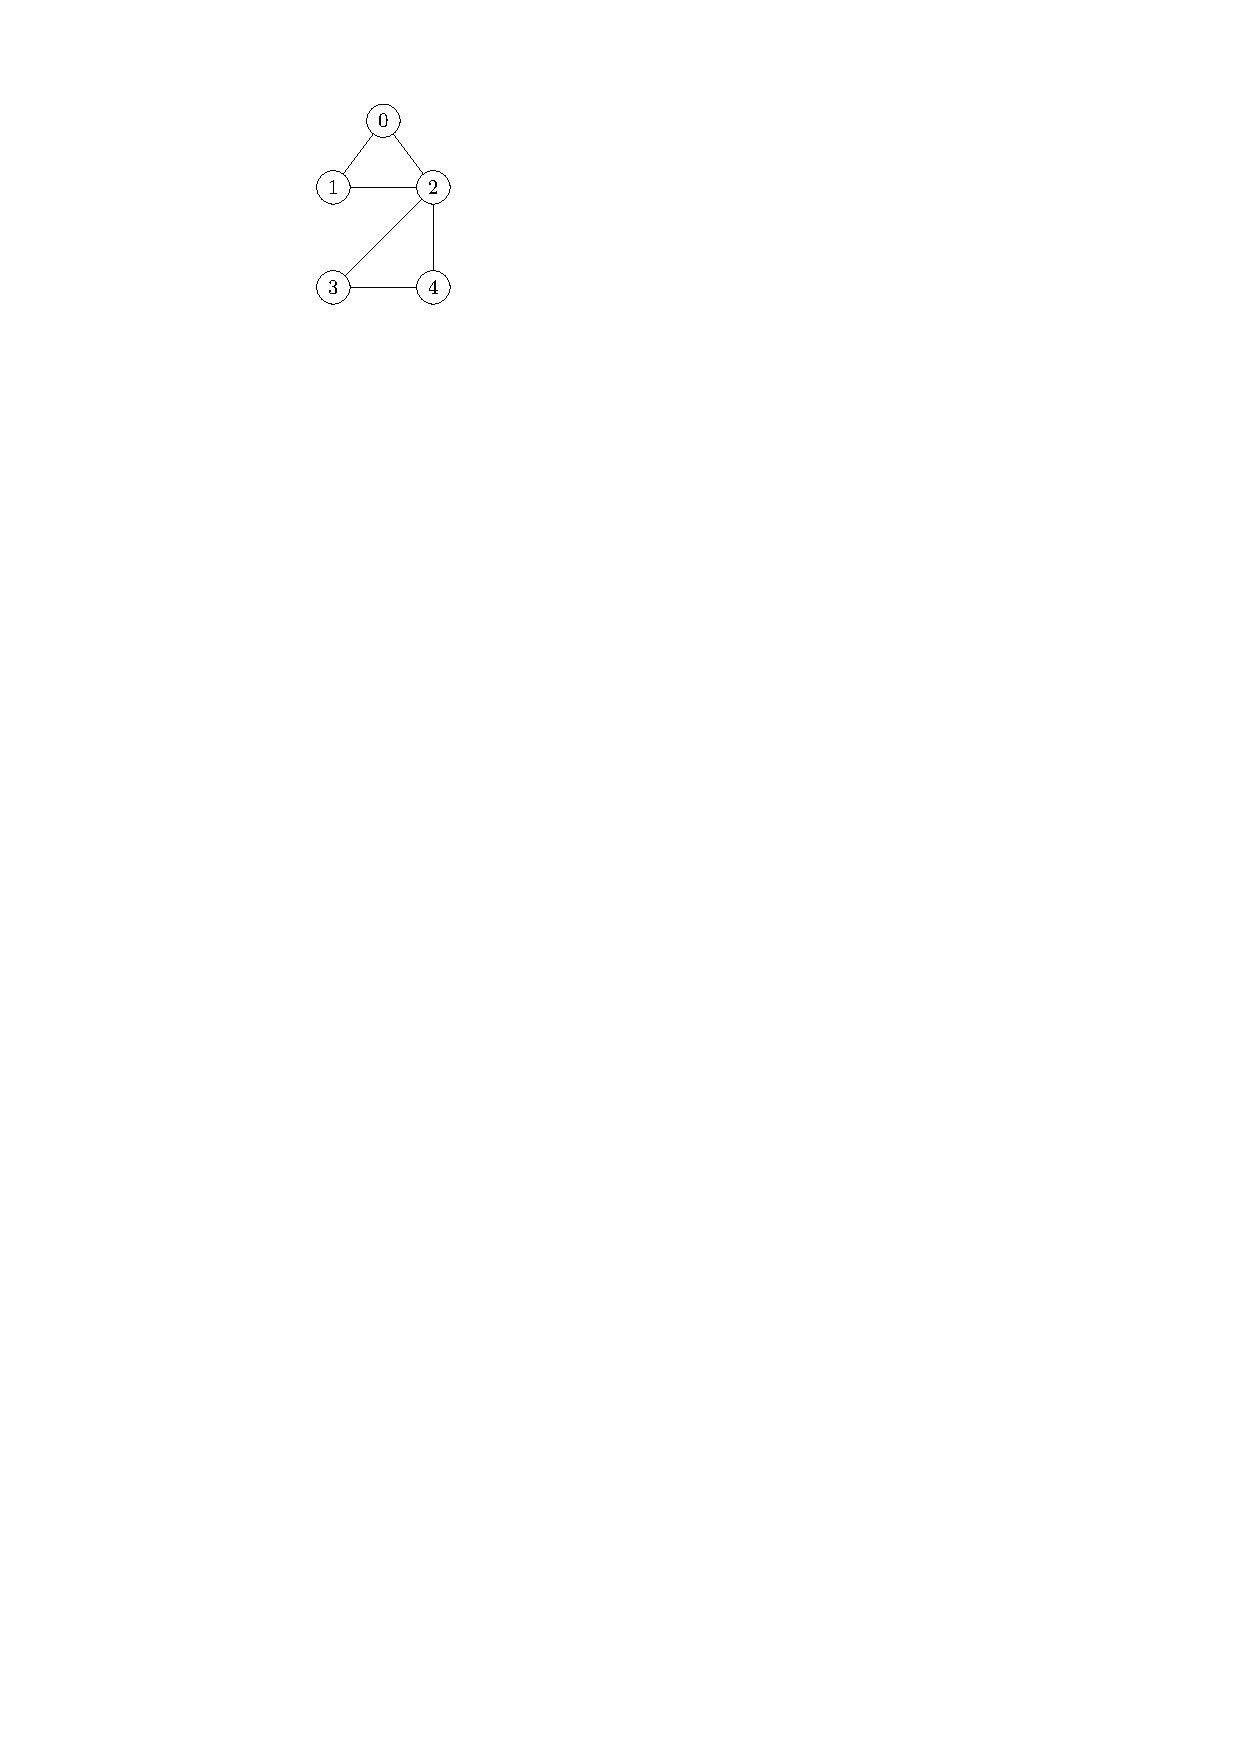
\includegraphics{graphExUndirected}
\end{minipage}
\begin{minipage}[c]{0.65\textwidth}
\begin{tabular}{|l|c|c|c|}\hline
\textbf{vertex sequence} & \textbf{walk?} & \textbf{path?} & \textbf{cycle?} \\ \hline
$0\, 3\, 2$                  & no  & no  &   \\
$0\, 1\, 2\, 3\, 4$          &     & yes & no  \\
$0\, 1\,  2\,  0$            & yes &     & yes  \\
$0 \, 1\,  0$                & yes & no  &  \\
$1\,  2\,  3\,  4\,  2\,  0$ &     &     &  \\
$3$							 & yes &     &  \\
\hline
\end{tabular}
\end{minipage}
\end{Boxample}

\begin{Boxample}[7]
Show that if there is a walk from $u$ to $v$, then we can find a path from $u$ to $v$.
\end{Boxample}

\begin{Definition} 
In a graph, the \defnfont{degree} of a vertex $v$ is the number of edges meeting $v$. 
In a digraph, the \defnfont{outdegree} of a node $v$ is the number of out-neighbours of $v$, 
and the \defnfont{indegree} of $v$ is the number of in-neighbours of $v$.

A node of indegree $0$ is called a \defnfont{source} and a node of outdegree $0$ is called a \defnfont{sink}.
\end{Definition}

%\begin{Boxample}[3]
%Prove that in a digraph, the sum of all outdegrees equals the sum of all 
%indegrees. What is the analogous statement for a graph? 
%\end{Boxample}

\begin{Definition}
The \defnfont{distance} from $u$ to $v$ in $G$, denoted by $d(u,v)$, is 
the number of arc on a shortest path from $u$ to $v$. If no path from $u$ to $v$ exists, the 
distance is undefined (or $+\infty$).
\end{Definition}

For graphs, we have $d(u,v) = d(v,u)$ for all vertices $u, v$. 

\begin{Boxample}[2]
Give the following distances for the digraph on the left.\\
\newline
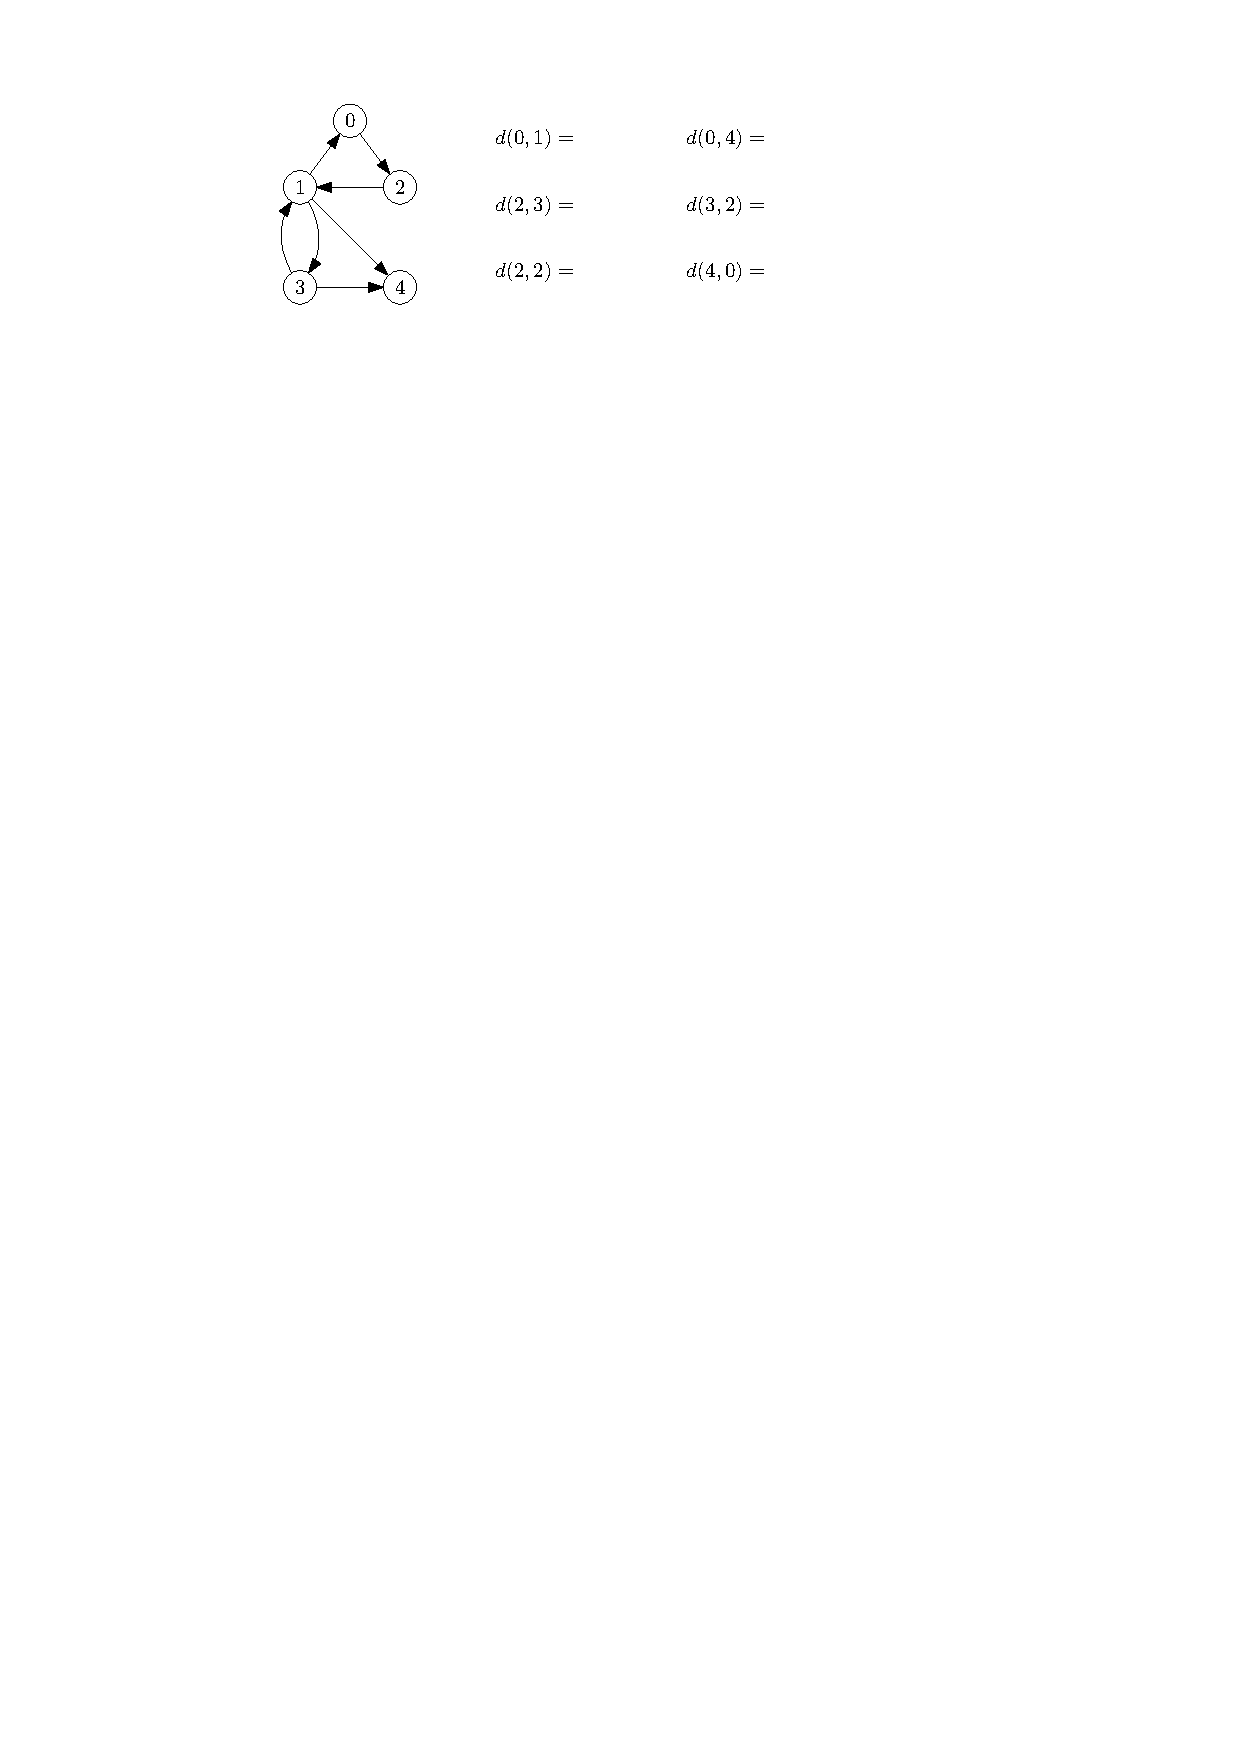
\includegraphics{distancesDirected}
\newline

Why are the values $d(4, v)$ not defined unless $v = 4$?
\end{Boxample}

\section{Creating new digraphs from old ones}
There are several ways to create new digraphs from old ones.
One way is to delete nodes and arcs in such a way that the 
resulting object is still a digraph (no arcs missing endpoints).

\begin{Definition}
A \defnfont{subdigraph} of a digraph $G = (V, E)$ is a digraph $G' = (V', E')$ 
where $V'\subseteq V$ and $E'\subseteq E$. 
A \defnfont{spanning} subdigraph is one with $V' = V$; that is, it contains all nodes.
\end{Definition}

\begin{Boxample}
A digraph (left) with a subdigraph (middle) and a spanning subdigraph (right).
\begin{center}
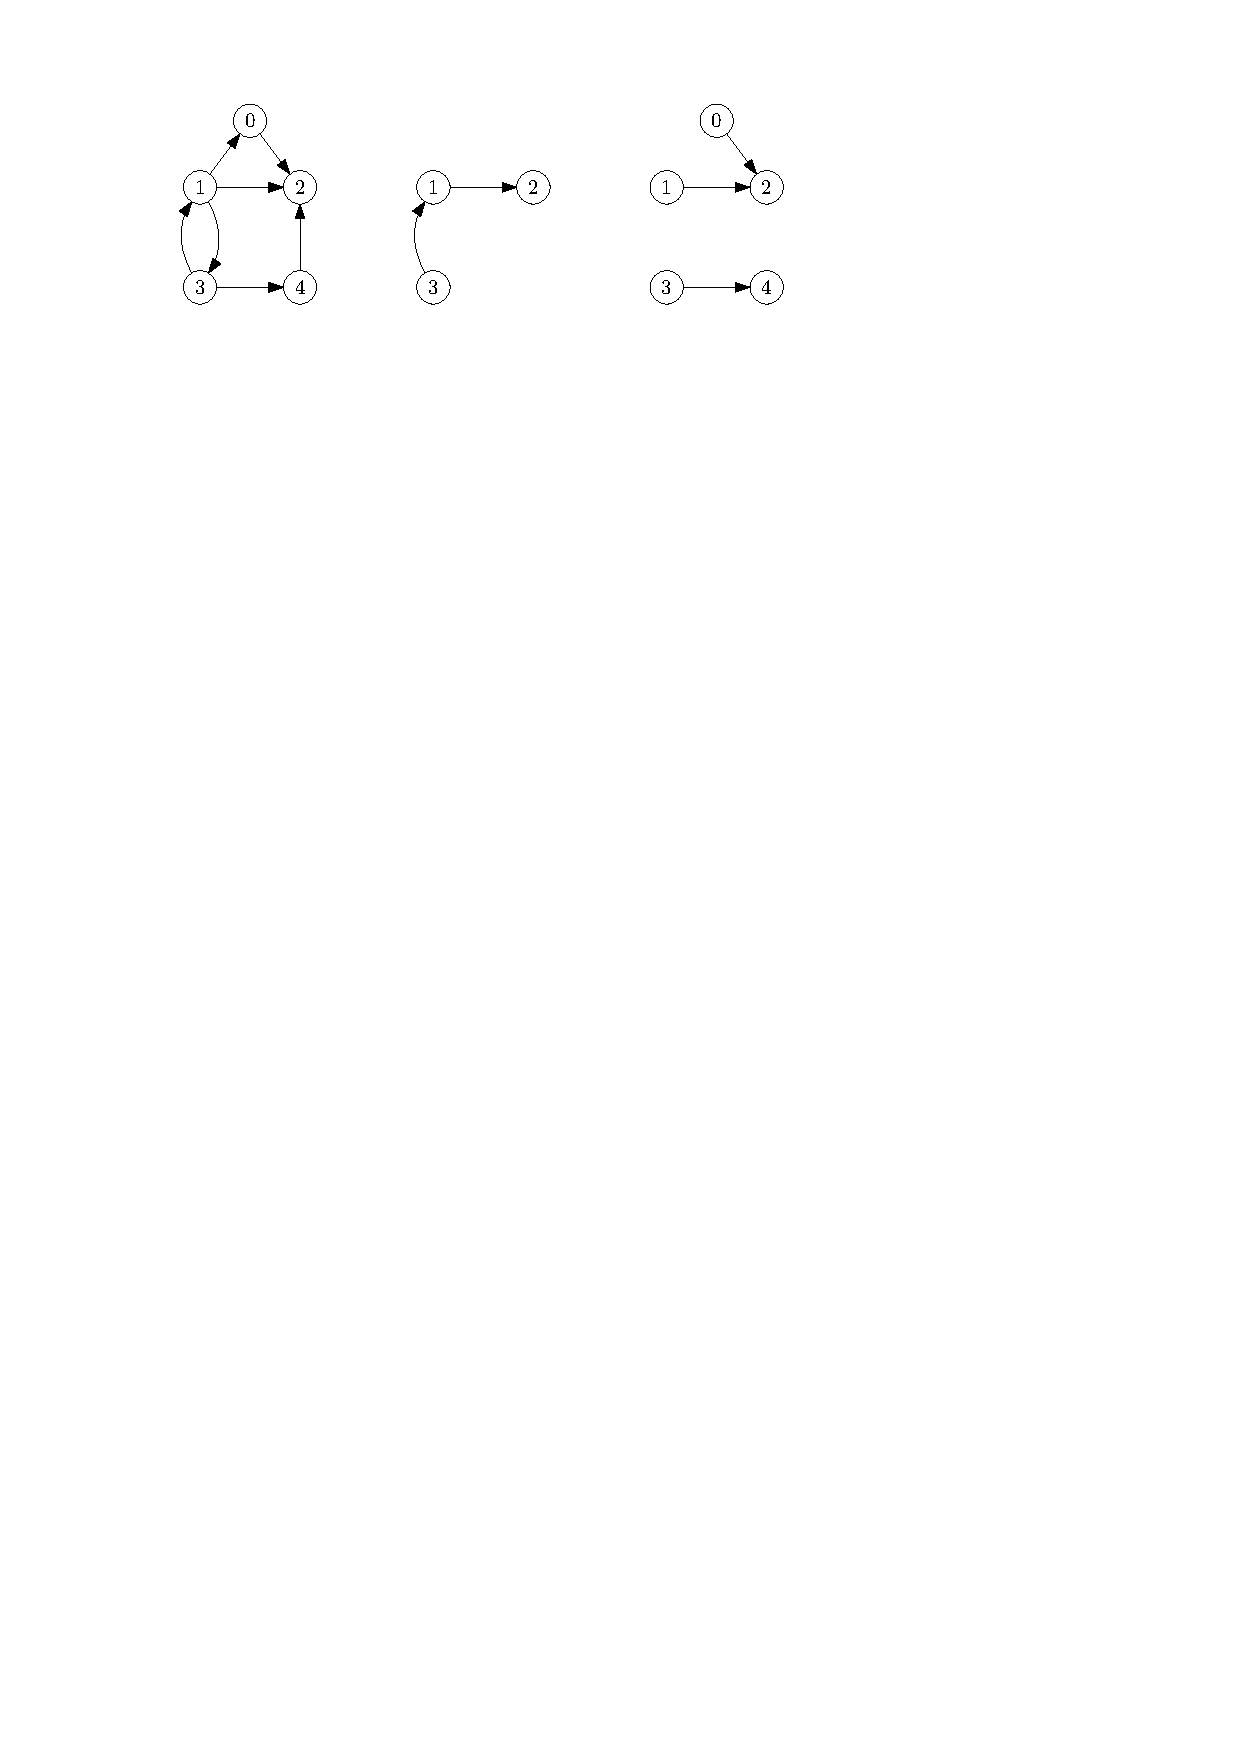
\includegraphics{graphExSubSpan} 
\end{center}
\end{Boxample}

\begin{Definition}
The subdigraph \defnfont{induced} by a subset $V'$ of $V$ is the digraph
$G' = (V', E')$ where $E' = \set{(u, v) \in E \mid u \in V' \mbox{ and } v\in V'}$.
\end{Definition}

\begin{Boxample}
For the digraph shown on the left, draw the subdigraph induced by  \set{1, 2, 3} on the right.
\begin{center}
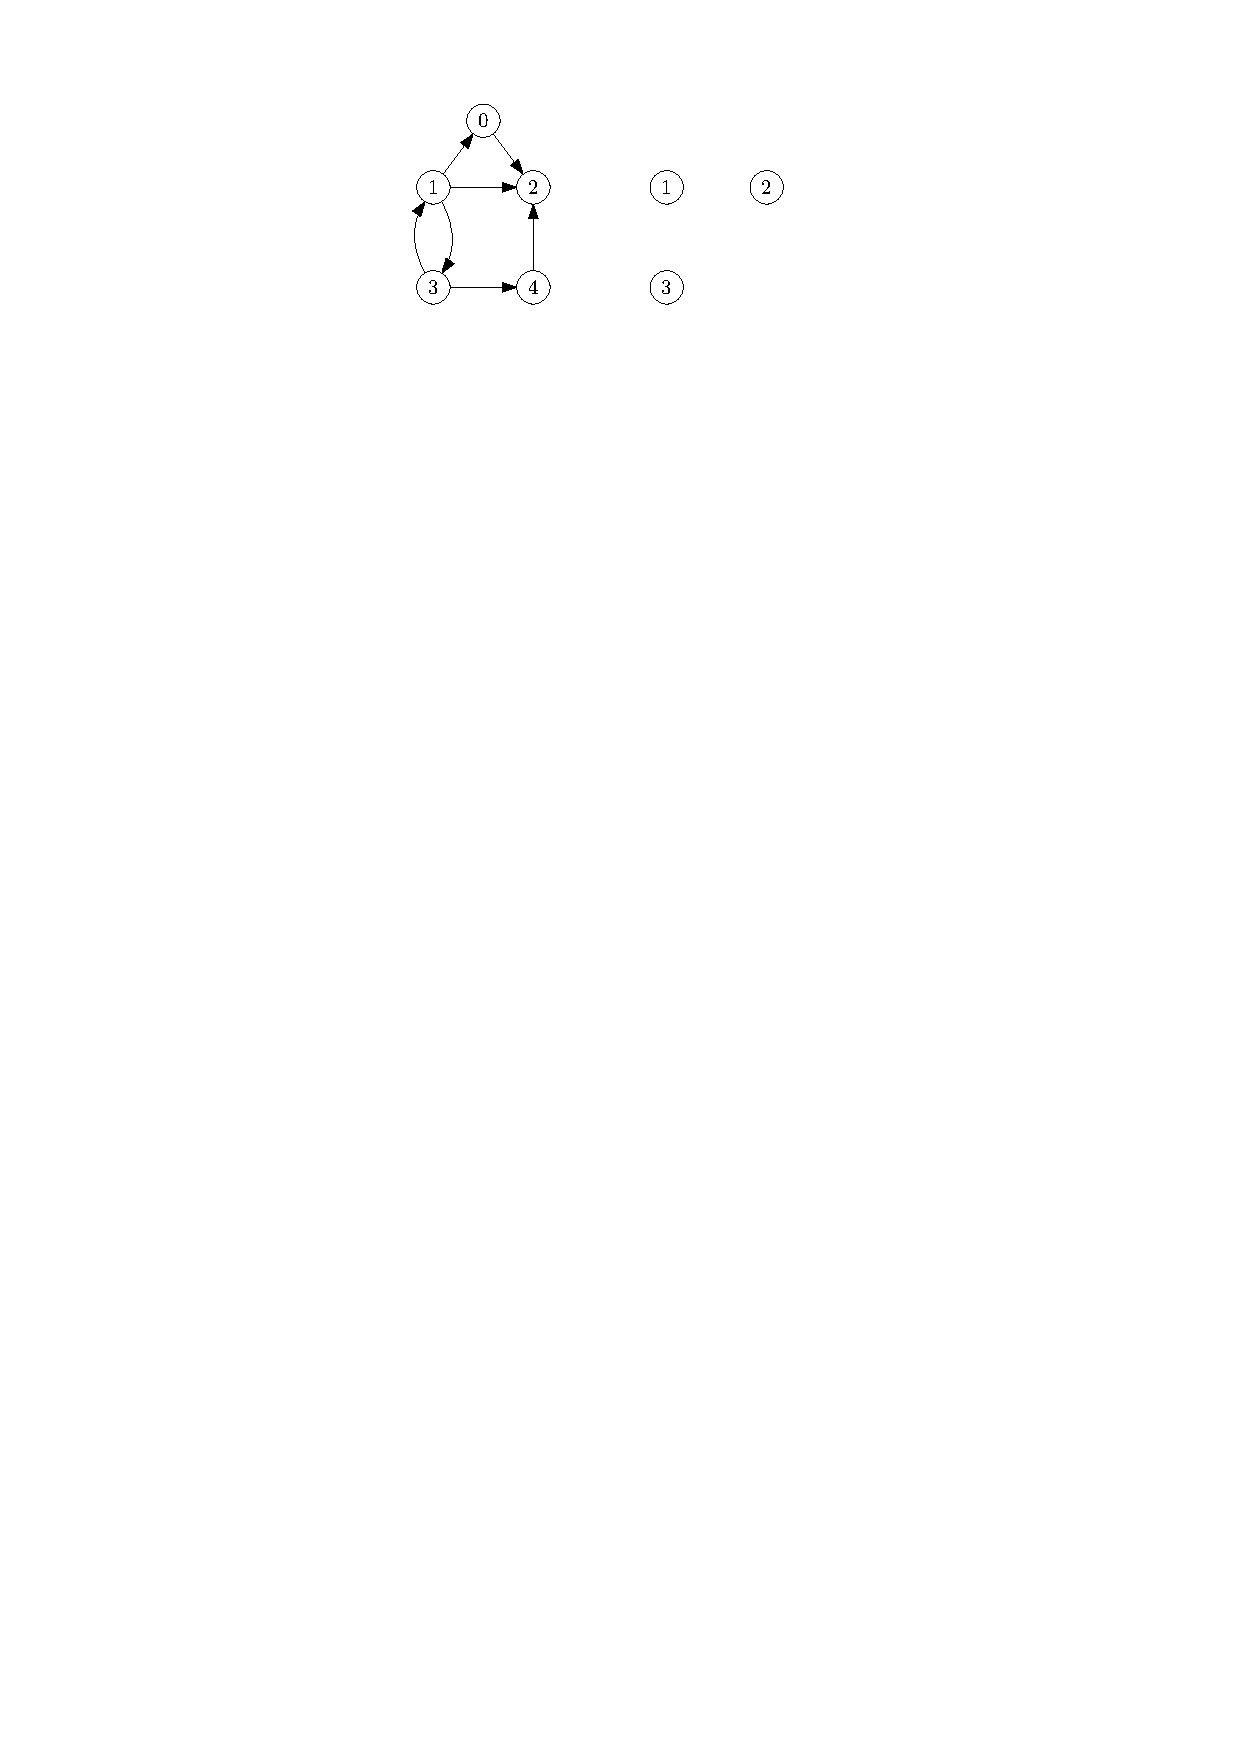
\includegraphics{graphExInducedEx}
\end{center}
\end{Boxample}

\begin{Definition}
The \defnfont{reverse digraph} of the digraph $G = (V, E)$, is the digraph $G_r = (V, E')$ where $(u, v)\in E'$ if and only if $(v, u)\in E$.
\end{Definition}

\begin{Boxample}\label{exr:compute-reverse}
Digraph $G$ and its reverse $G_r$. We simply reverse all the arrows.
\begin{center}
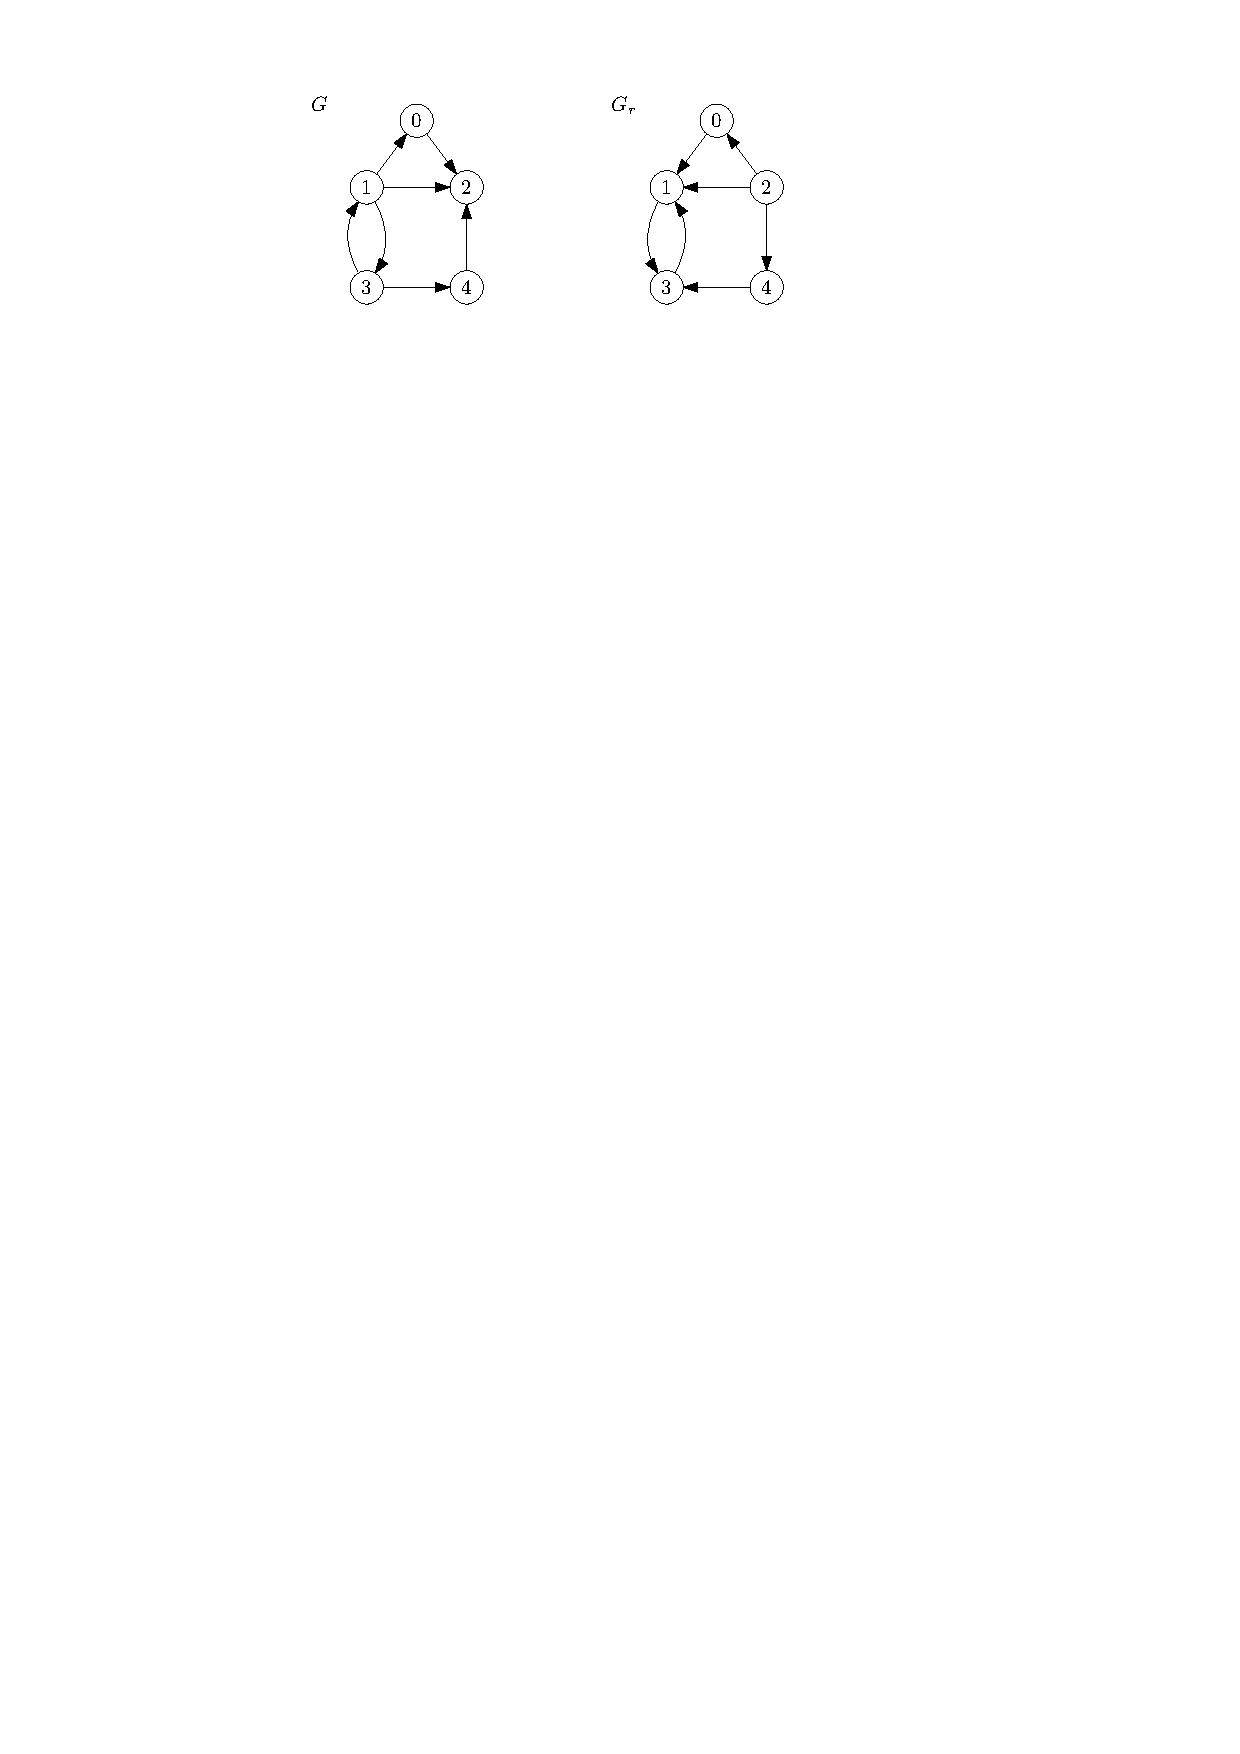
\includegraphics{graphExReverse}
\end{center}
\end{Boxample}

It is sometimes useful to ignore the direction of arcs in a digraph to find the associated `underlying graph'.

\begin{Definition} 
The \defnfont{underlying graph} of a digraph $G = (V, E)$ is the graph 
$G' = (V, E')$ where $E' = \set{\{u, v\} \mid (u, v)\in E}$.
\end{Definition}

Note that the underlying graph does not have multiple edges even when there are arcs $(u, v)$ and $(v, u)$. 
In that case, only one edge joins $u$ and $v$ in the underlying graph $G'$.  
%This is because $\{u, v\}$ and $\{v, u\}$ are equal as sets, so appear only once in the set $E'$.

\begin{Boxample}
Draw the underlying graph $G'$ of the digraph $G$.
\begin{center}
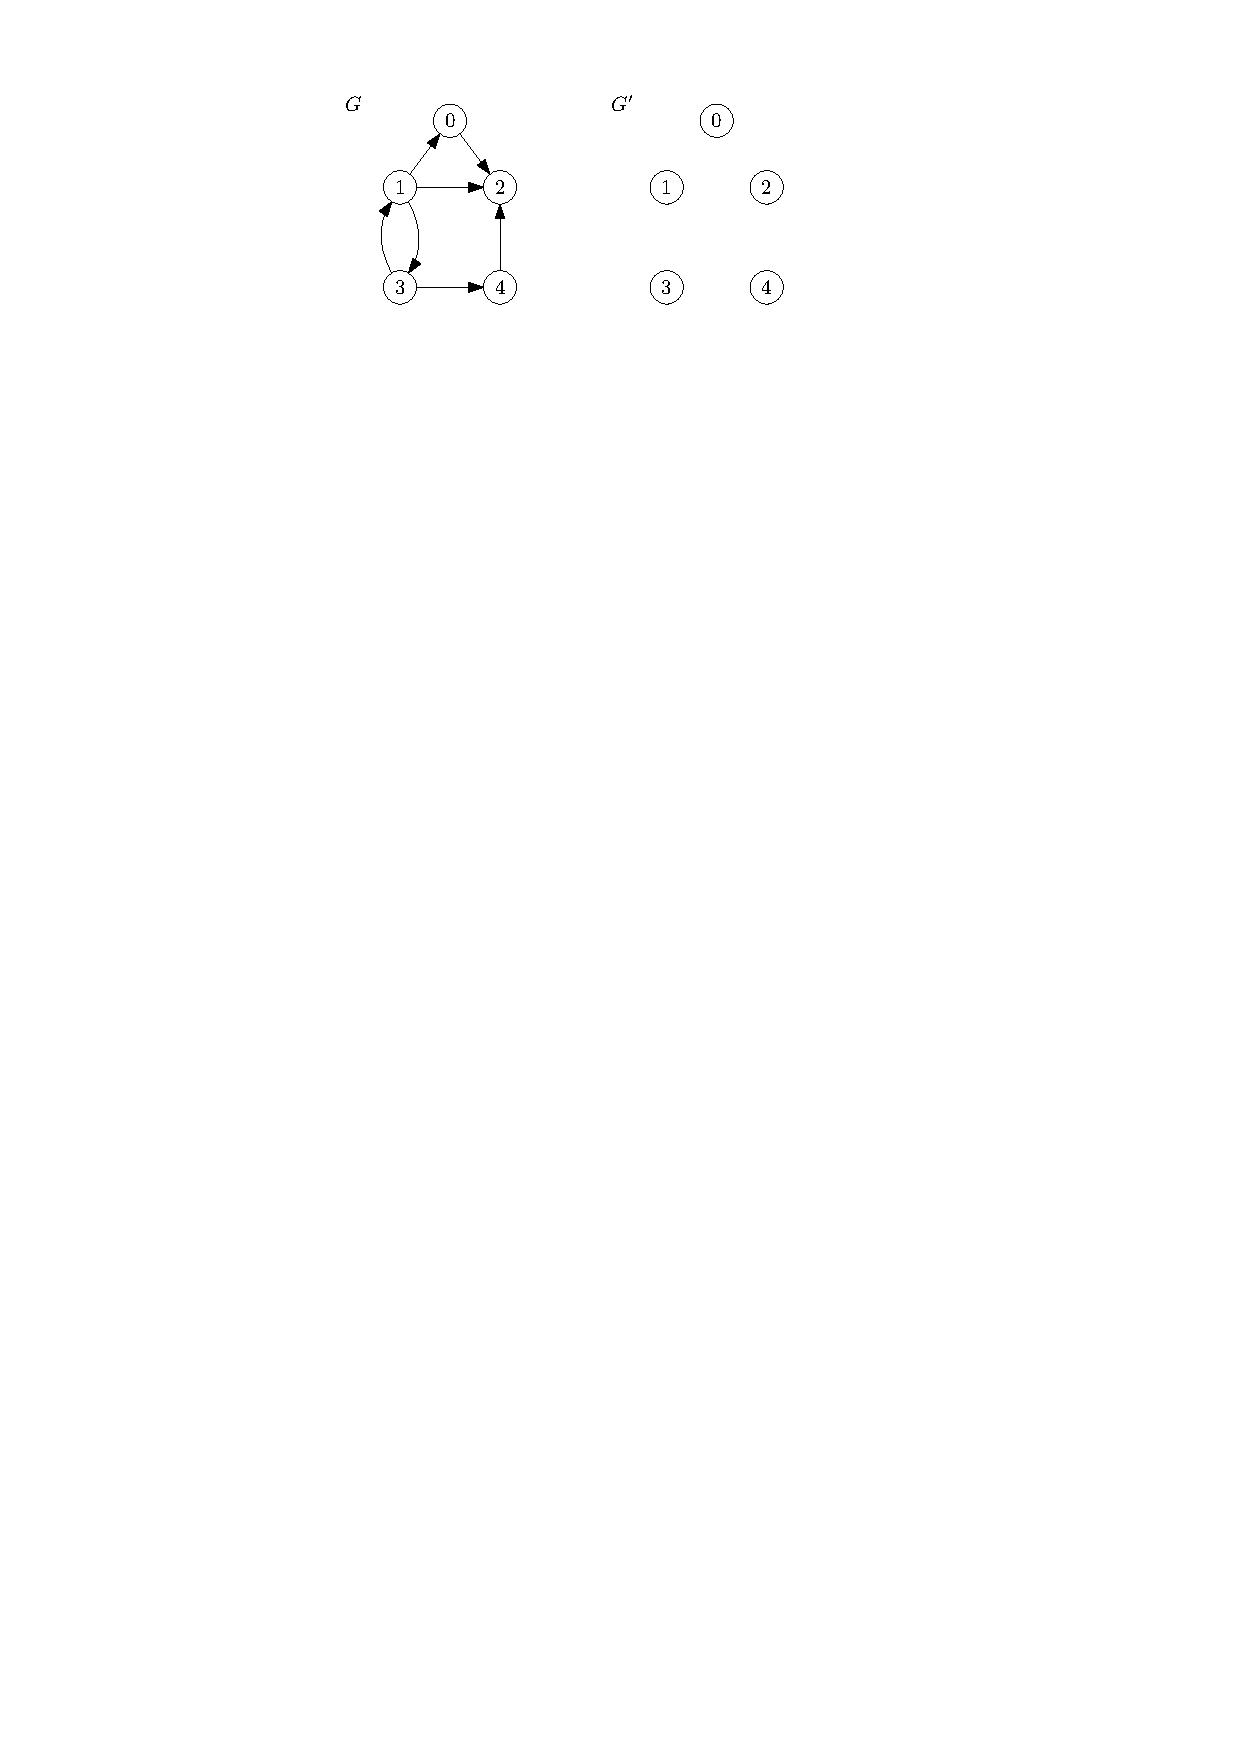
\includegraphics{graphExUnderlyingEx}
\end{center}
%Note that there should be only a single edge between vertices 1 and 3.
\end{Boxample}

\begin{Definition} 
We can combine two or more digraphs $G_1, G_2$, \ldots $G_k$ into a
single graph where the vertices of each $G_i$ are completely disjoint from
each other and no arc goes between the different $G_i$. The constructed
graph $G$ is called the \defnfont{graph union}, where $V(G) = V(G_1) \cup
V(G_2) \cup \ldots \cup V(G_k)$ and $E(G) = E(G_1) \cup E(G_2) \cup \ldots
\cup E(G_k)$.
\end{Definition}

%\begin{Boxample}[3] \label{ex:distbound}
%Let $G$ be a digraph of order $n$ and $u, v$ nodes of $G$. 
%Show that $d(u, v) \leq n - 1$ if there is a walk from $u$ to $v$.
%\end{Boxample}

%\begin{Boxample}[3] \label{ex:sparse-deg}
%Prove that in a sparse digraph, the average indegree of a node is $O(1)$, 
% while in a dense digraph, the average indegree of a node is $\Omega(n)$.
%\end{Boxample}

 

\chapter{Graph data structures} \label{sec:graph-reps} %---------------------------------
When representing a digraph in a computer, we assume
that it has nodes given in a fixed order with the
\boldfont{convention that the nodes are labelled $0, 1, \dots, n - 1$}.

\begin{Definition}
Let $G$ be a digraph of order $n$. The \defnfont{adjacency matrix} of $G$
is the $n\times n$ Boolean matrix (often encoded with $0$'s and $1$'s)
such that entry $(i, j)$ is true if and only if there is an arc from the
node $i$ to node $j$.
\end{Definition}

\begin{Definition}
For a digraph $G$ of order $n$, an \defnfont{adjacency lists}
representation is a sequence of $n$ sequences, $L_0, \dots, L_{n-1}$. 
Sequence $L_i$ contains all nodes of $G$ that are out-neighbours of node $i$.
\end{Definition}

%In the adjacency lists representation, only the out-neighbours of node $i$ are listed in the sequence $L_i$. 
In the adjacency lists representation, $L_i$ may or may not be sorted in order of increasing node number. 
Our \boldfont{convention is to sort them whenever convenient}. 
Many implementations do \boldfont{not} enforce this convention.

\begin{Boxample}
A graph and its adjacency matrix and adjacency list.\\
\begin{center}
\begin{minipage}[c]{0.3\textwidth}
\centering
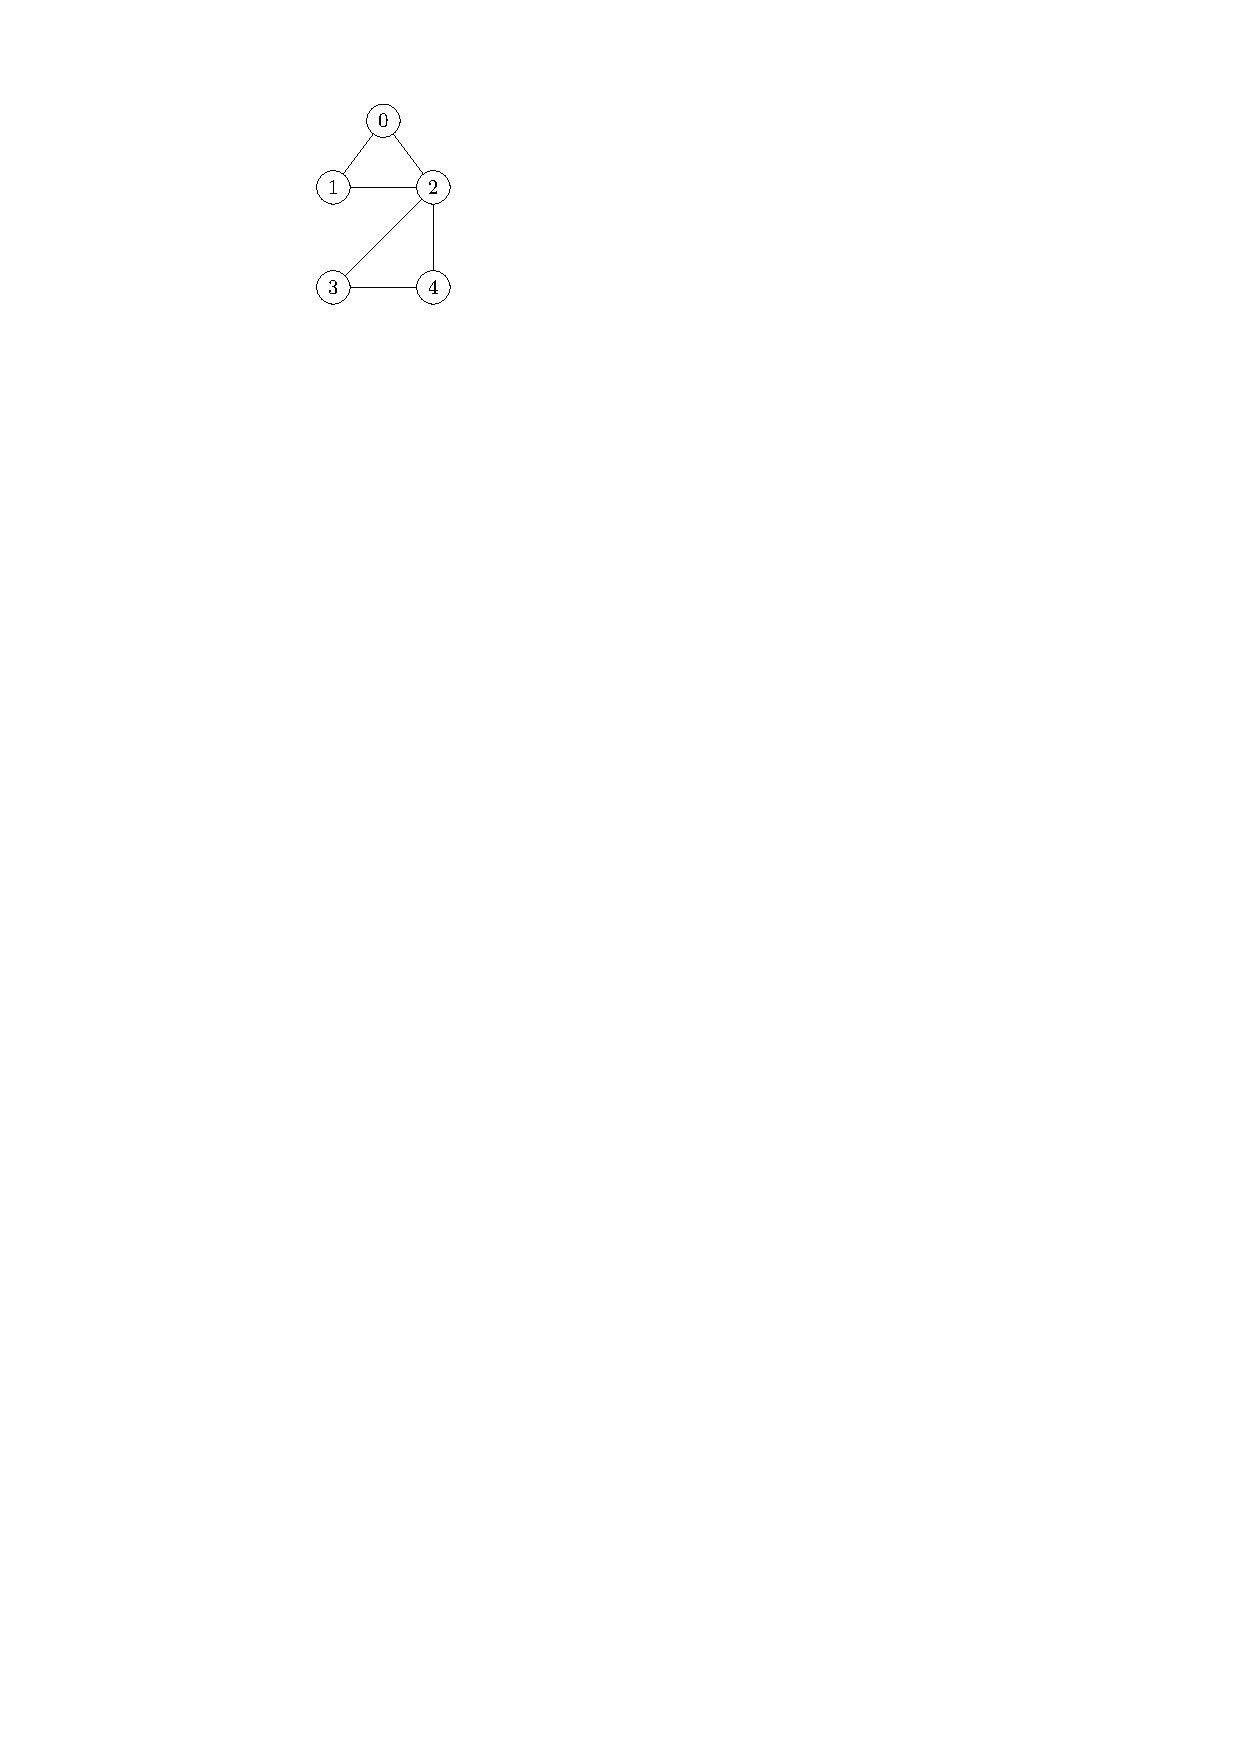
\includegraphics{graphExUndirected}
\end{minipage}
\begin{minipage}[c]{0.65\textwidth}
$\quad \left[
	\begin{matrix}
	0 & 1 & 1 & 0 & 0 \\
	1 & 0 & 1 & 0 & 0 \\
	1 & 1 & 0 & 1 & 1 \\
	0 & 0 & 1 & 0 & 1 \\
	0 & 0 & 1 & 1 & 0 
	\end{matrix}
\right] 
\qquad \qquad
\lightgraybox{
	\begin{array}{c|cccc}
	0 & 1 & 2 &   &   \\
	1 & 0 & 2 &   &   \\
	2 & 0 & 1 & 3 & 4 \\
	3 & 2 & 4 &   &   \\
	4 & 2 & 3 &   &   \\
	\end{array}
}$
\end{minipage}
\end{center}
Notice that the number of $1$'s in a row in the adjacency matrix is the outdegree of the corresponding node, 
while the number of $1$'s in a column is the indegree.
\end{Boxample}



\begin{Boxample}
\label{ex:adjlist}
A digraph and its adjacency matrix and adjacency list.\\
\begin{center}
\begin{minipage}[c]{0.3\textwidth}
\centering
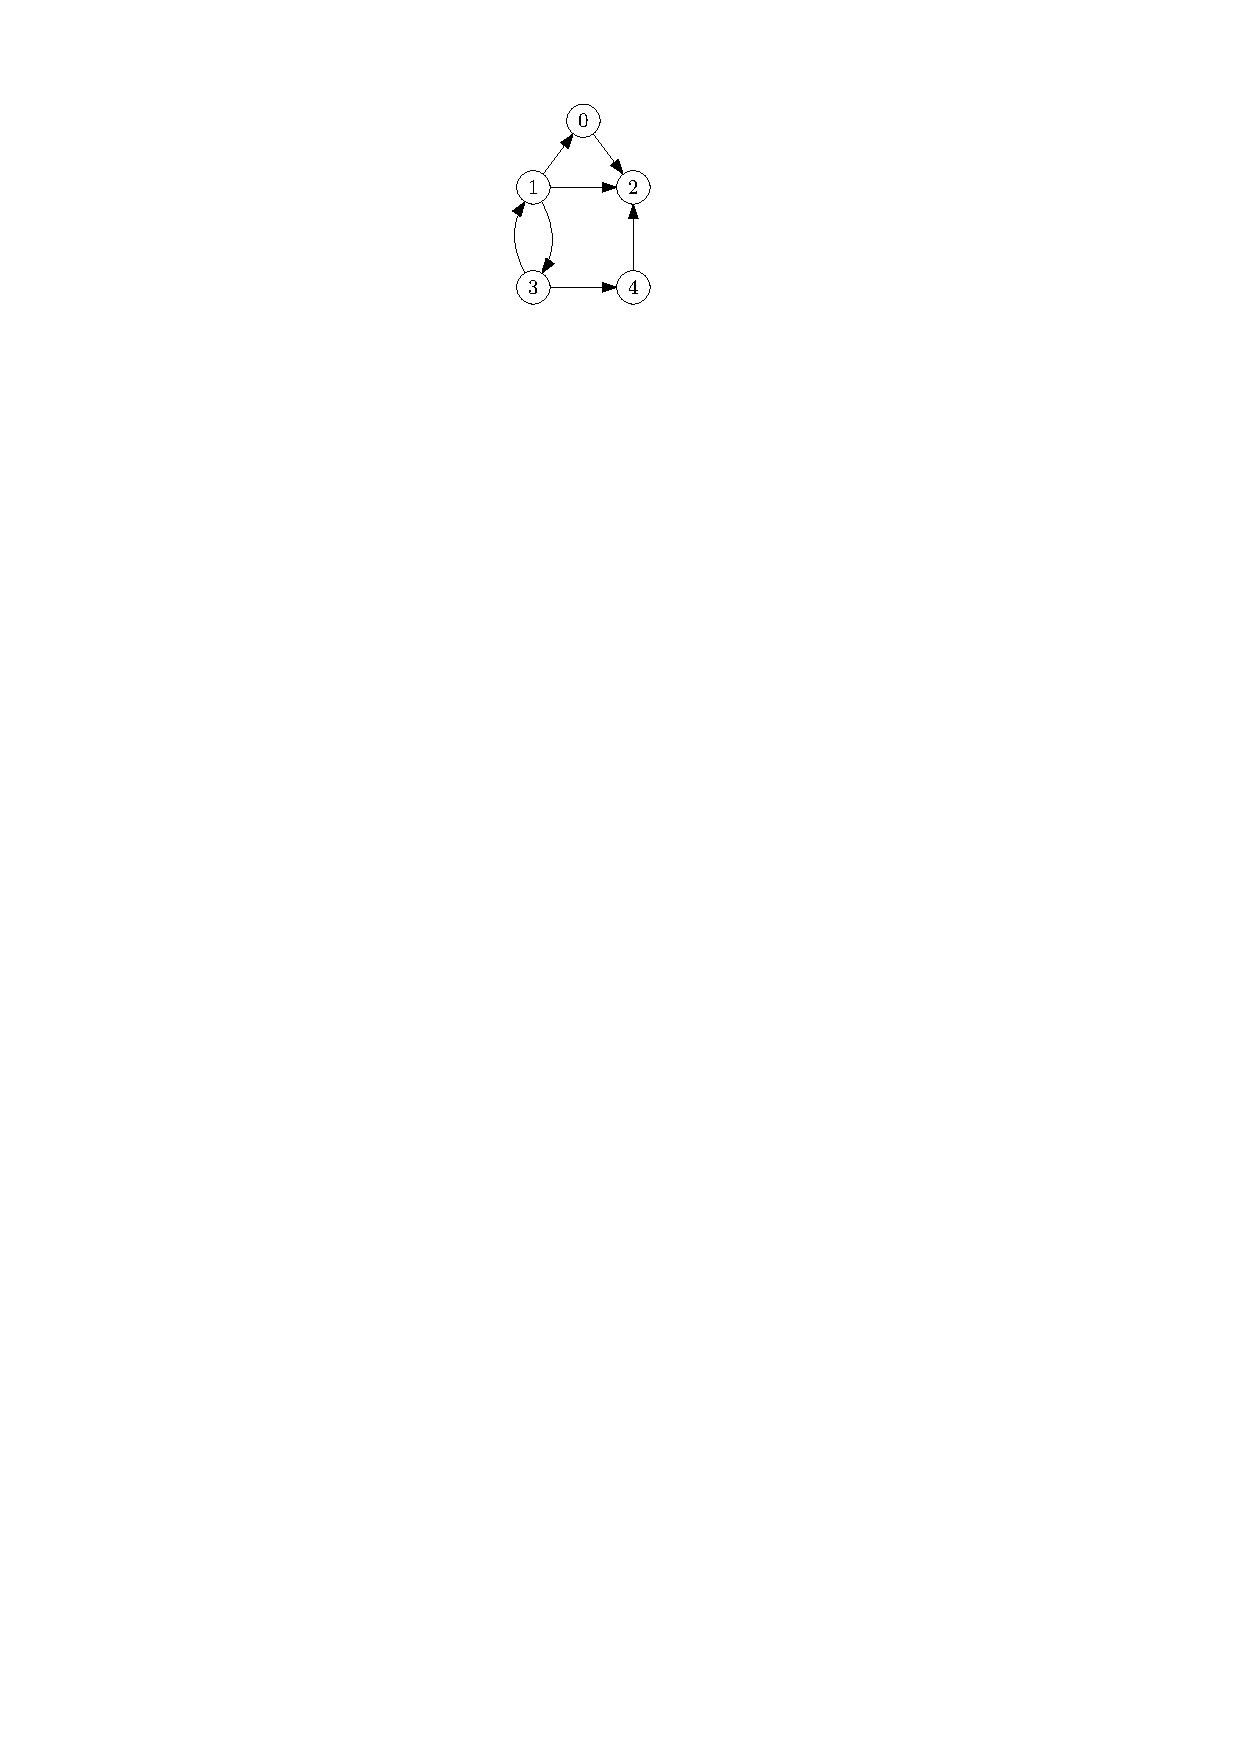
\includegraphics{graphExDirected}
\end{minipage}
\begin{minipage}[c]{0.65\textwidth}
$\quad\left[
	\begin{matrix}
	0 & 0 & 1 & 0 & 0 \\
	1 & 0 & 1 & 1 & 0 \\
	0 & 0 & 0 & 0 & 0 \\
	0 & 1 & 0 & 0 & 1 \\
	0 & 0 & 1 & 0 & 0 
	\end{matrix}
\right]
\qquad \qquad
\lightgraybox{
	\begin{array}{c|ccc}
	0 & 2  \\
	1 & 0 & 2 & 3  \\
	2  \\
	3 & 1 & 4  \\
	4 & 2 \\
	\end{array}
}$
\end{minipage}
\end{center}
An empty sequence occurs in the adjacency list where a node has no out-neighbours (for example, sequence $2$). 
\end{Boxample}

Sometimes the node labels in adjacency lists are omitted, so the digraph in \cref{ex:adjlist} would be written as:
$$\lightgraybox{
	\begin{array}{ccc}
	2 &   &   \\
	0 & 2 & 3 \\
	  &   &   \\
	1 & 4 &   \\
	2 &   &   \\
	\end{array}
}$$

\begin{Boxample}[2]
Give the adjacency matrix of the digraph below.

	\vspace{1cm}
	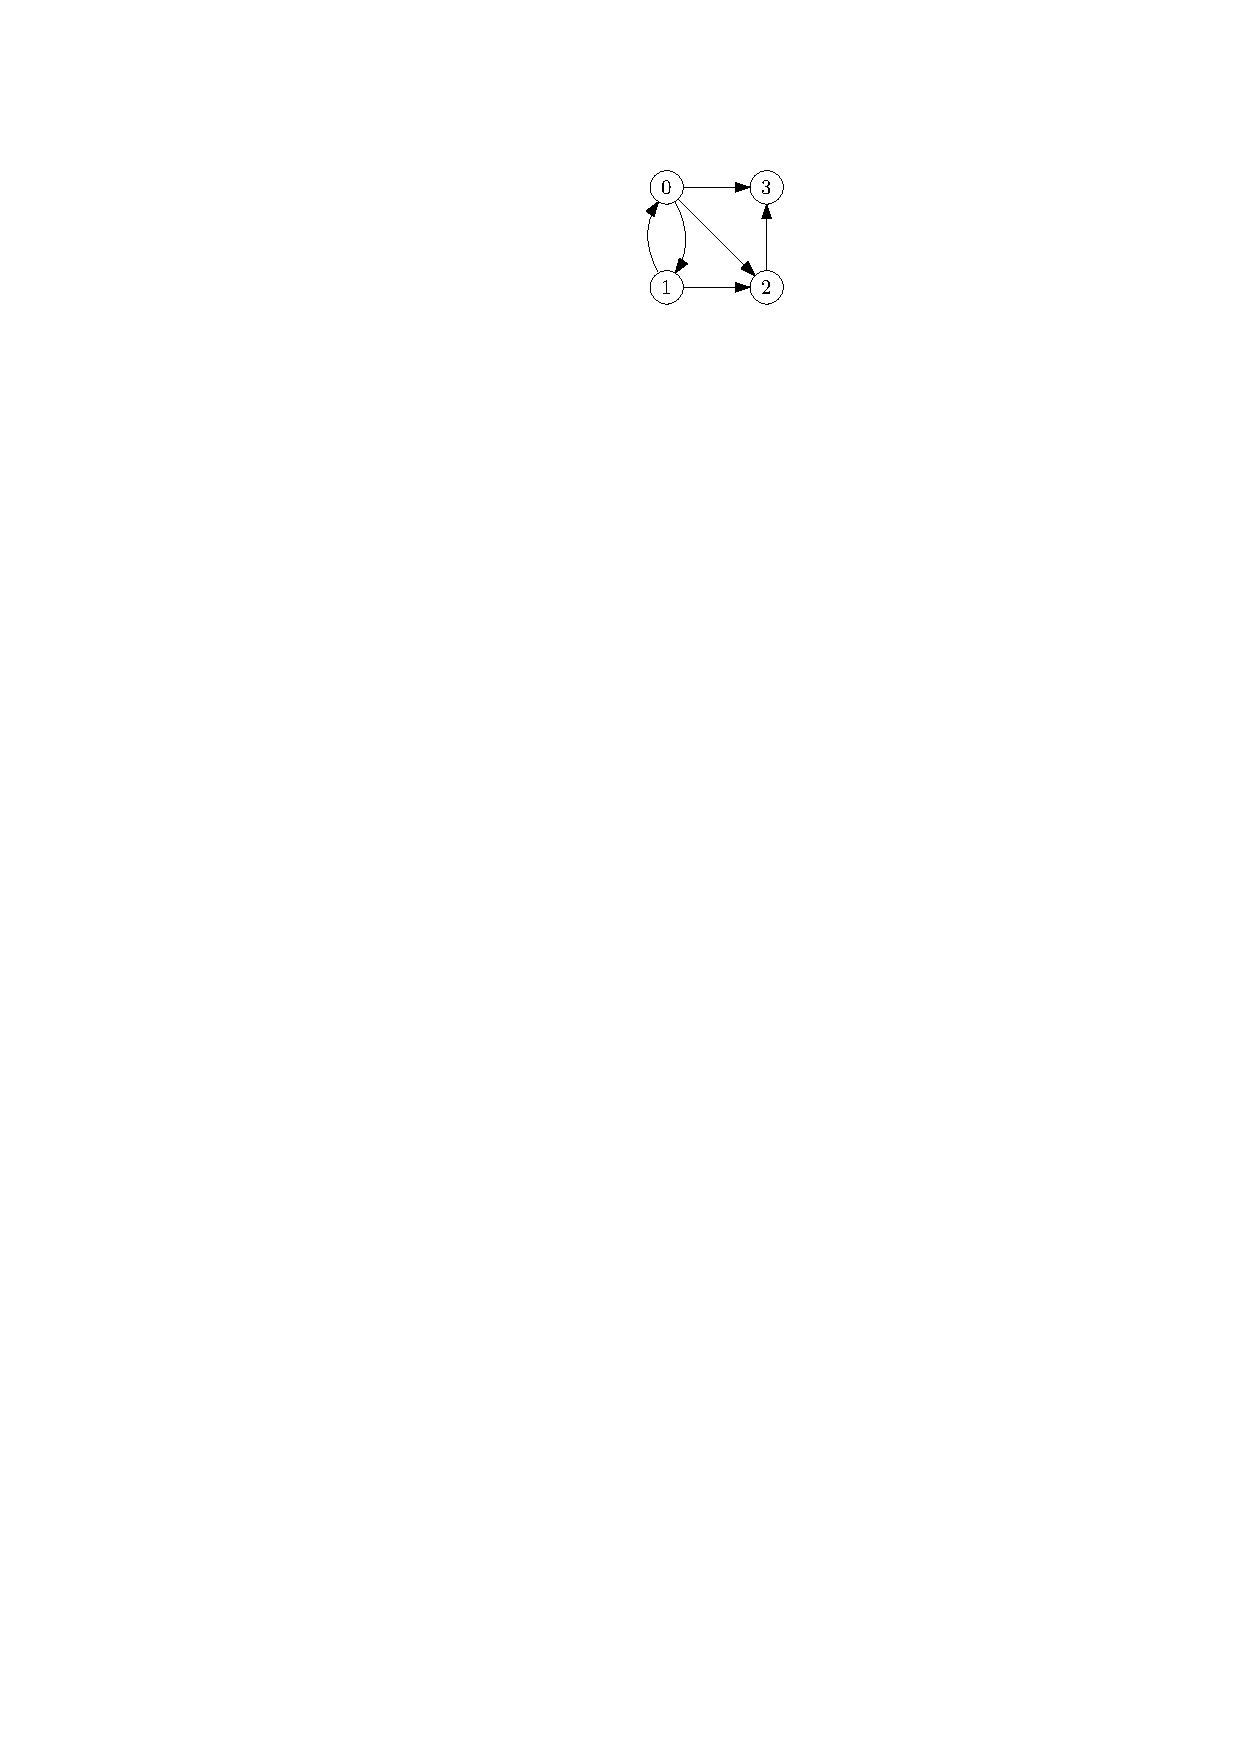
\includegraphics{graphEx4}
	\vspace{1cm}
	
Draw the digraph corresponding to the given adjacency matrix.

	\vspace{1cm}
	$\left[
	\begin{matrix}
	0 & 1 & 0 & 1 & 0 \\
	1 & 0 & 0 & 0 & 1 \\
	0 & 1 & 0 & 0 & 1 \\
	1 & 0 & 1 & 0 & 0 \\
	0 & 0 & 1 & 1 & 0 
	\end{matrix}
	\right]$
\end{Boxample}

\begin{Boxample}[1] \label{ex:drawadjlist}
Give the adjacency lists of the digraph below.

	\vspace{1cm}
	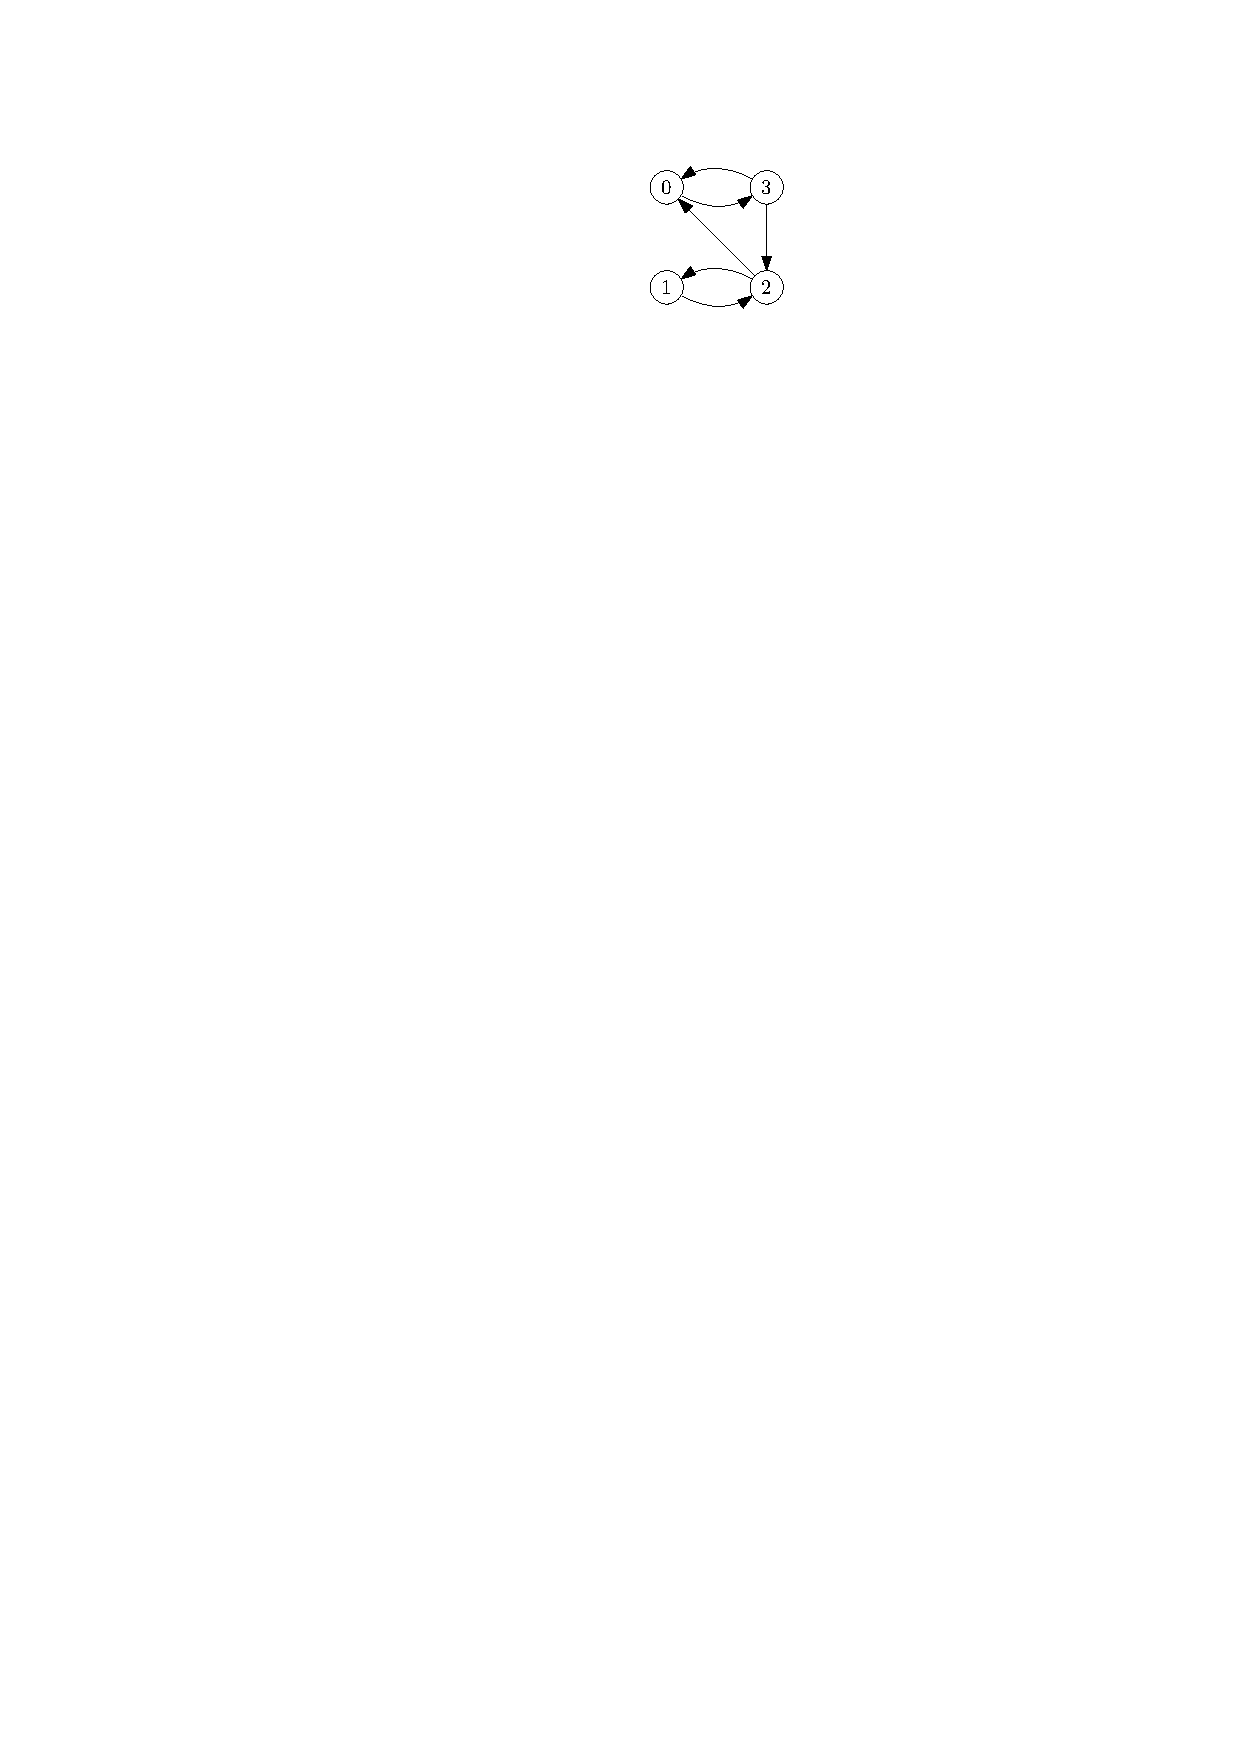
\includegraphics{graphEx5}
	\vspace{1cm}
	
Draw the digraph corresponding to the given adjacency lists.

	\vspace{1cm}
	$\lightgraybox{\begin{array}{c|ccc}
	0 & 1 & 2  \\
	1 & 3  \\
	2  \\
	3 & 0 & 1 & 2 \\
	\end{array}}$
\end{Boxample}

\section{Representing multiple graphs in a single file}
We can store several digraphs one after the other in a single file as follows: 
\begin{itemize}
  \item We have a single line giving the order at the beginning of each digraph.
  \item If the order is $n$ then the next $n$ lines give the adjacency matrix 
  or adjacency lists representation of the digraph. Node labels are omitted.
  \item The end of the file is marked with a line denoting a digraph of order $0$.
\end{itemize}

\begin{Boxample} 
The two digraphs on the left could be put in a single file:\\

\begin{minipage}[c]{0.5\textwidth}
\centering
	$\lightgraybox{\begin{array}{c|c}
	0 & 2  \\
	1 & 0  \\
	2 & 1 \\
	\end{array}}$
	
	\vspace{1cm}
	$\lightgraybox{\begin{array}{c|ccc}
	0 & 1 & 2  \\
	1 & 3  \\
	2  \\
	3 & 0 & 1 & 2 \\
	\end{array}}$
\end{minipage}
\begin{minipage}[c]{0.5\textwidth}
$$
\lightgraybox{
	\begin{array}{ccc}
	3 &   &   \\
	2 &   &   \\
	0 &   &   \\
	1 &   &   \\
	4 &   &   \\
	1 & 2 &   \\
	3 &   &   \\
	  &   &   \\
	0 & 1 &  2 \\
	0 &   &   \\
	\end{array}
}
$$
\end{minipage}
\end{Boxample}


\section{Using other structures to represent graphs}

Other specialized digraph representations may be used take advantage of
special structure in a family of digraphs for improved storage or access time. For such specialized
purposes they may be better adjacency matrices or lists.

For example, trees can be stored more efficiently (c.f. \cref{sec:heapsort}).  
\begin{itemize}
\item A general rooted tree of $n$ nodes can be stored in array $\pred$ of size $n$. 
\item $\pred[i]$ is the parent of node $i$. 
\item The root has no parent, so assign it \texttt{null} or $-1$ if we number nodes from $0$
to $n-1$ in the usual way. 
\item This is a form of adjacency lists, using in-neighbours instead of out-neighbours.
\end{itemize}

\begin{Boxample}[4]
Draw the tree represented by the array $$\pred = [-1,0,0,1,2,2,2,3]\text{.}$$
\end{Boxample}

%\begin{Boxample}[5]
%Consider the digraph $G$ whose nodes are the integers from $1$ to $12$
%inclusive and such that $(i, j)$ is an arc if and only if $i$ is a
%proper divisor of $j$ (that is, $i$ divides $j$ and $i \neq j$).
%Write down the adjacency matrix representation of $G$ and of $G_r$.
%\end{Boxample}

\section{Implementation of digraph ADT} \label{sec:graphadtimpl}
An adjacency matrix is simply a matrix which is an array of arrays. 

Adjacency lists are a list of lists. 
There are several ways in which a list can be implemented, for
example by an array, or singly- or doubly-linked lists using pointers.  
These have different properties, for example, accessing the middle element is $\Theta(1)$ for an array but $\Theta(n)$ for a linked list. 
Searching for a value that may or may not be in the list requires sequential search
and takes $\Theta(n)$ time in the worst case. 
%
We do not consider other data structures (e.g. heaps) that can be used to represent lists. 

\section{Complexity of basic digraph operations}
The basic operations we consider are checking for the existence of an arc between two nodes, finding the outdegree of a node, 
finding the indegree of a node, adding an arc between two nodes, deleting an arc between two nodes, adding a node, and deleting a node. 

For the two data structures, consider the steps we need to carry out various basic operations and the cost of all steps. 

\begin{Boxample}
Compare the matrix and lists data structures for checking whether arc $(i,j)$ exists.\\
	\boldfont{Adjacency matrix representation}: 
	We need to check whether element $(i,j)$ is 1. 
	This requires accessing an array element twice, to first find the $i$th array then its $j$th element. 
	Each array access is in $\Theta(1)$ so overall it is in $\Theta(1)$.
	
	\boldfont{Adjacency lists representation}: We need to search for $j$ in list $i$. 
	The complexity then depends on the length of list $i$. 
	List $i$ is length $d$ where $d$ is the outdegree of node $i$ so searching for $j$ is in $\Theta(d)$. 
	But how large is $d$? 
	Even when the graph is sparse, it could still be the case that $d$ is $O(n)$,
	though typically in a sparse graph $d$ is $O(1)$.  
	In a dense graph $d$ is $O(n)$.
\end{Boxample}

\begin{Boxample}[3]
Compare the matrix/lists data structures for deleting a node.\\
	\boldfont{Adjacency matrix representation}: \vspace{3cm}
%	We must delete a row and column, and move up some elements so there are no gaps in the matrix. 
%	In the worst case, we need to move all remaining elements in the matrix 
%	and since there are now $(n-1)$s rows and columns, it takes time $\Theta(n^2)$.
	
	\boldfont{Adjacency lists representation}: 
%	We must remove a list and also all references to the deleted node in other lists. 
%	This requires scanning each list for the offending entry and deleting it. 
%	We thus need to visit $n$ lists and the combined length of all remaining lists which is (in the worst case) $m$, 
%	requiring $\Theta(n + m)$ work in total.
\end{Boxample}

\cref{tbl:basicOpsSteps} shows the steps required  
and \cref{tbl:basicOpsPerformance} the time required for basic graph operations 
when using adjacency matrix or lists representations.  
Performance for the adjacency list representation is based on using doubly linked lists.

\begin{table}[H]
\centering
\caption{Steps required to perform basic digraph operations by data structure.}
\label{tbl:basicOpsSteps}
\begin{tabular}{|l|l|l|}
\hline
\textbf{Operation} & \textbf{Adjacency Matrix} & \textbf{Adjacency Lists} \\
\hline
arc $(i, j)$ exists? & is entry $(i,j)$ 0 or 1  & find $j$ in  list $i$ \\
\hline
outdegree  of $i$ & scan row, count $1$'s & size of  list  $i$\\
\hline
indegree of $i$ & scan column,  count $1$'s & for $j\neq i$, find $i$ in list $j$ \\
\hline
add arc $(i, j)$ & change entry $(i ,j)$ & insert $j$ in list $i$ \\
\hline
delete arc $(i, j)$ & change entry $(i ,j)$ & delete $j$ from list $i$ \\
\hline
add node & create new row and column & add new list at end\\
\hline
delete node $i$ & delete row/column $i$  & delete list $i$ \\
& shuffle other entries & for $j\neq i$, delete  $i$ from list $j$ \\
\hline
\end{tabular}
\end{table}

\begin{table}[H]
\centering
\caption{Comparative worst-case performance of adjacency lists and matrices.}
\label{tbl:basicOpsPerformance}
\begin{tabular}{|l|c|c|}
\hline
\textbf{Operation} 	& \textbf{Matrix} & \textbf{Lists} \\
\hline
arc $(i, j)$ exists? & $\Theta(1)$  & $\Theta(d)$ \\
\hline
outdegree  of $i$ 	& $\Theta(n)$ & $\Theta(1)$ \\
\hline
indegree of $i$ 	& $\Theta(n)$ &  $\Theta(n+m)$ \\
\hline
add arc $(i, j)$ 	& $\Theta(1)$ & $\Theta(1)$  \\
\hline
delete arc $(i, j)$ & $\Theta(1)$  & $\Theta(d)$  \\
\hline
add node 			& $\Theta(n)$ & $\Theta(1)$  \\
\hline
delete node $i$ 	& $\Theta(n^2)$  & $\Theta(n+m)$  \\
\hline
\end{tabular}
\end{table}

Using lists, apparently similar problems like finding the outdegree ($\Theta(1)$) and indegree ($\Theta(n+m)$)
have very different time complexity. 
%\begin{itemize}
%  \item Finding the outdegree with lists merely requires accessing
%the correct list (constant time) plus finding the size of that list
%(constant time). 
%\item Finding the indegree with lists requires
%scanning all lists except one ($n-1$ of them), and looking at every arc in
%them, ($m$ arcs in the worst case), so taking time $\Theta(n+m)$. 
%\end{itemize}

Clearly finding all indegrees would be slow if we just used multiple calls to a method designed for getting the indegree of a single node. 

\begin{Boxample}[8]
Show that that sorted adjacency lists represention of the reverse digraph of $G$ can be found in time $\Theta(n+m)$ given the sorted adjacncy lits of $G$. Also show how this can be used to find indegrees for all nodes of $G$ in time $\Theta(n+m)$.
\end{Boxample}

\section{Space requirements}
The adjacency matrix representation requires $\Theta(n^2)$ storage 
as we simply need a matrix of $n^2$ bits. 

At first guess we might say adjacency lists require $\Theta(n + m)$ storage, 
since we need $n$ lists and the combined length of all the lists is $m$.
But node numbers require more than one bit of storage each; the number $k$ uses about $\Theta(\log k)$ bits.
The average entry in a list is $\frac n 2$, so the total space requirement is more like $\Theta(n + m \log(n))$ 

\begin{Boxample}[4]
What is the storage requirement for a complete digraph on $n$ nodes, that is, a digraph where every possible arc
occurs?
\end{Boxample}

For small, sparse digraphs, lists use less space than a matrix, whereas for small
dense digraphs the space requirements are comparable. For large sparse
digraphs, a matrix can still be more efficient, but this happens rarely.

\begin{Boxample}[4]
Find a large sparse digraph where the matrix representation uses less space than the lists representation.
\end{Boxample}

The representation that is best will depend on the application and we cannot make general rules.  
We will mostly use adjacency lists, which are
clearly superior for many common tasks and generally better for sparse digraphs.

